\documentclass[tikz,border=6pt]{standalone}
\usepackage{tikz}
\usetikzlibrary{arrows.meta,calc}
\tikzset{
  planet/.style={draw,circle,minimum size=3cm,thick},
  object/.style={draw,circle,minimum size=6mm,thick},
  force/.style={-Latex,very thick}
}
\begin{document}
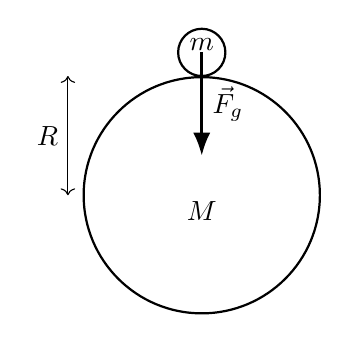
\begin{tikzpicture}
\node[planet] (M) at (0,0) {};
\node at (0,-0.2) {$M$};
\node[object,fill=white] (m) at ($(M.north)+(0,0.3)$) {};
\node at ($(m.center)+(0,0.1)$) {$m$};
\draw[force] (m.center) -- ($(M.center)+(0,0.5)$) node[midway,right] {$\vec{F}_g$};
\draw[<->] ($(M.center)+(-1.7,0)$) -- node[midway,left] {$R$} ($(M.north)+(-1.7,0)$);
\end{tikzpicture}
\end{document}
